\section{The hardware}
The aim of this chapter is to be able to built a speaker stand for the measurement. The requirement of the stand is that the stand shall be able to be fixed to the turntable. A drawing of the turntable is visualized in \autoref{fig:turn_table}


 \begin{figure}[H]
	\centering
	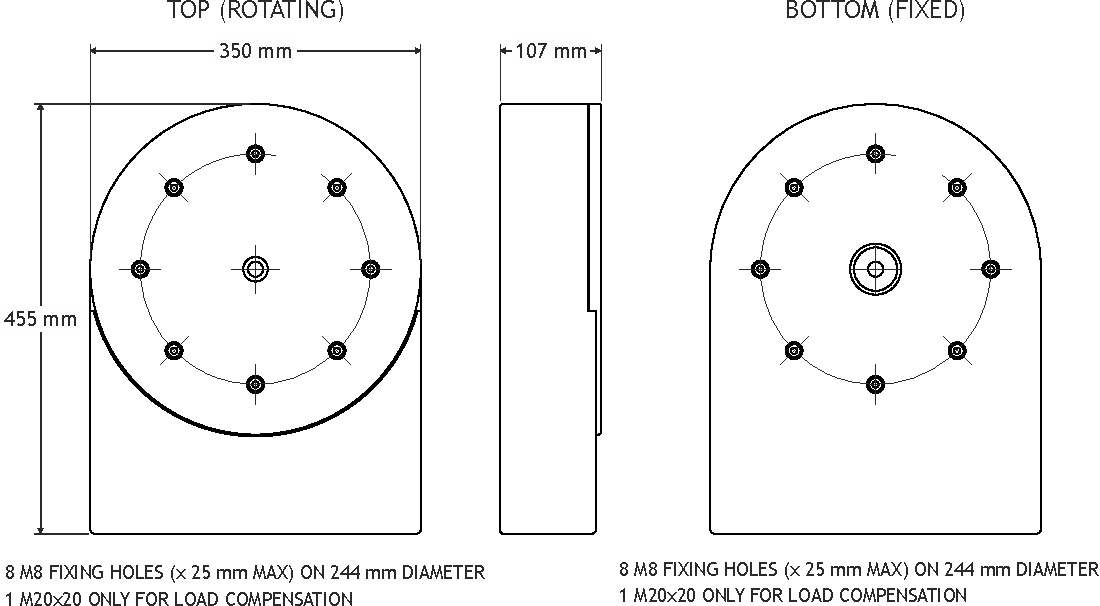
\includegraphics[width=1\textwidth]{ET250-3D_drawing}
	\caption{A drawing of the Outline turntable ET 250-3D \citep{ET250-3D}}
		\label{fig:turn_table}
\end{figure}



The drawing of the turntable in \autoref{fig:turn_table} shows that the turn part of the turntable only have a diameter of \SI{350}{\milli\meter}. The speaker construction shall at least have a diameter of \SI{1.1}{\meter} such that the acoustical center can be separated be \SI{400}{\milli\meter}. To achieve more stability for the speaker stand, the rotational part of the turntable is extended by a circular wood plate with a diameter of \SI{800}{\milli\meter}. The circular plate is bolted to the eight M8 screw holes on  \autoref{fig:turn_table}. \\
To be able to mount the speaker on the wood plate a metal speaker stand will de designed. The design of the speaker stand have to be as minimal as possible to avoid reflection from the speaker, but is shall be rigid enough the hold the speaker in a still position. Therefore it is been chosen to use squared metal pipe for the construction. The construction will be build such that the speaker is raised at least \SI{1}{\meter} from the wood plate, to avoid reflections\\
The placement of the speaker cabinet has to be adjustable, because the speaker cabinet is placed close to each other, and the infliction of the cabinet is unknown. Therefore the metal frame will be divided intro a bottom part and three stand part. The resend for splitting the stand and the bottom frame is such that the stand is adjustable in the frame part. To make the adjustable features possible, the bottom part is build out of squared pipe with a width of \SI{45}{\milli\meter} where the stand part is build out of squared pipe with a width of \SI{40}{\milli\meter}. This enable the stand to be slided intro the bottom part. To make higher stability, the outer \SI{400}{\milli\meter} of bottom part is cutted as a 'u' pipe as visualized in \autoref{fig:botom_u}

 \begin{figure}[H]
	\centering
	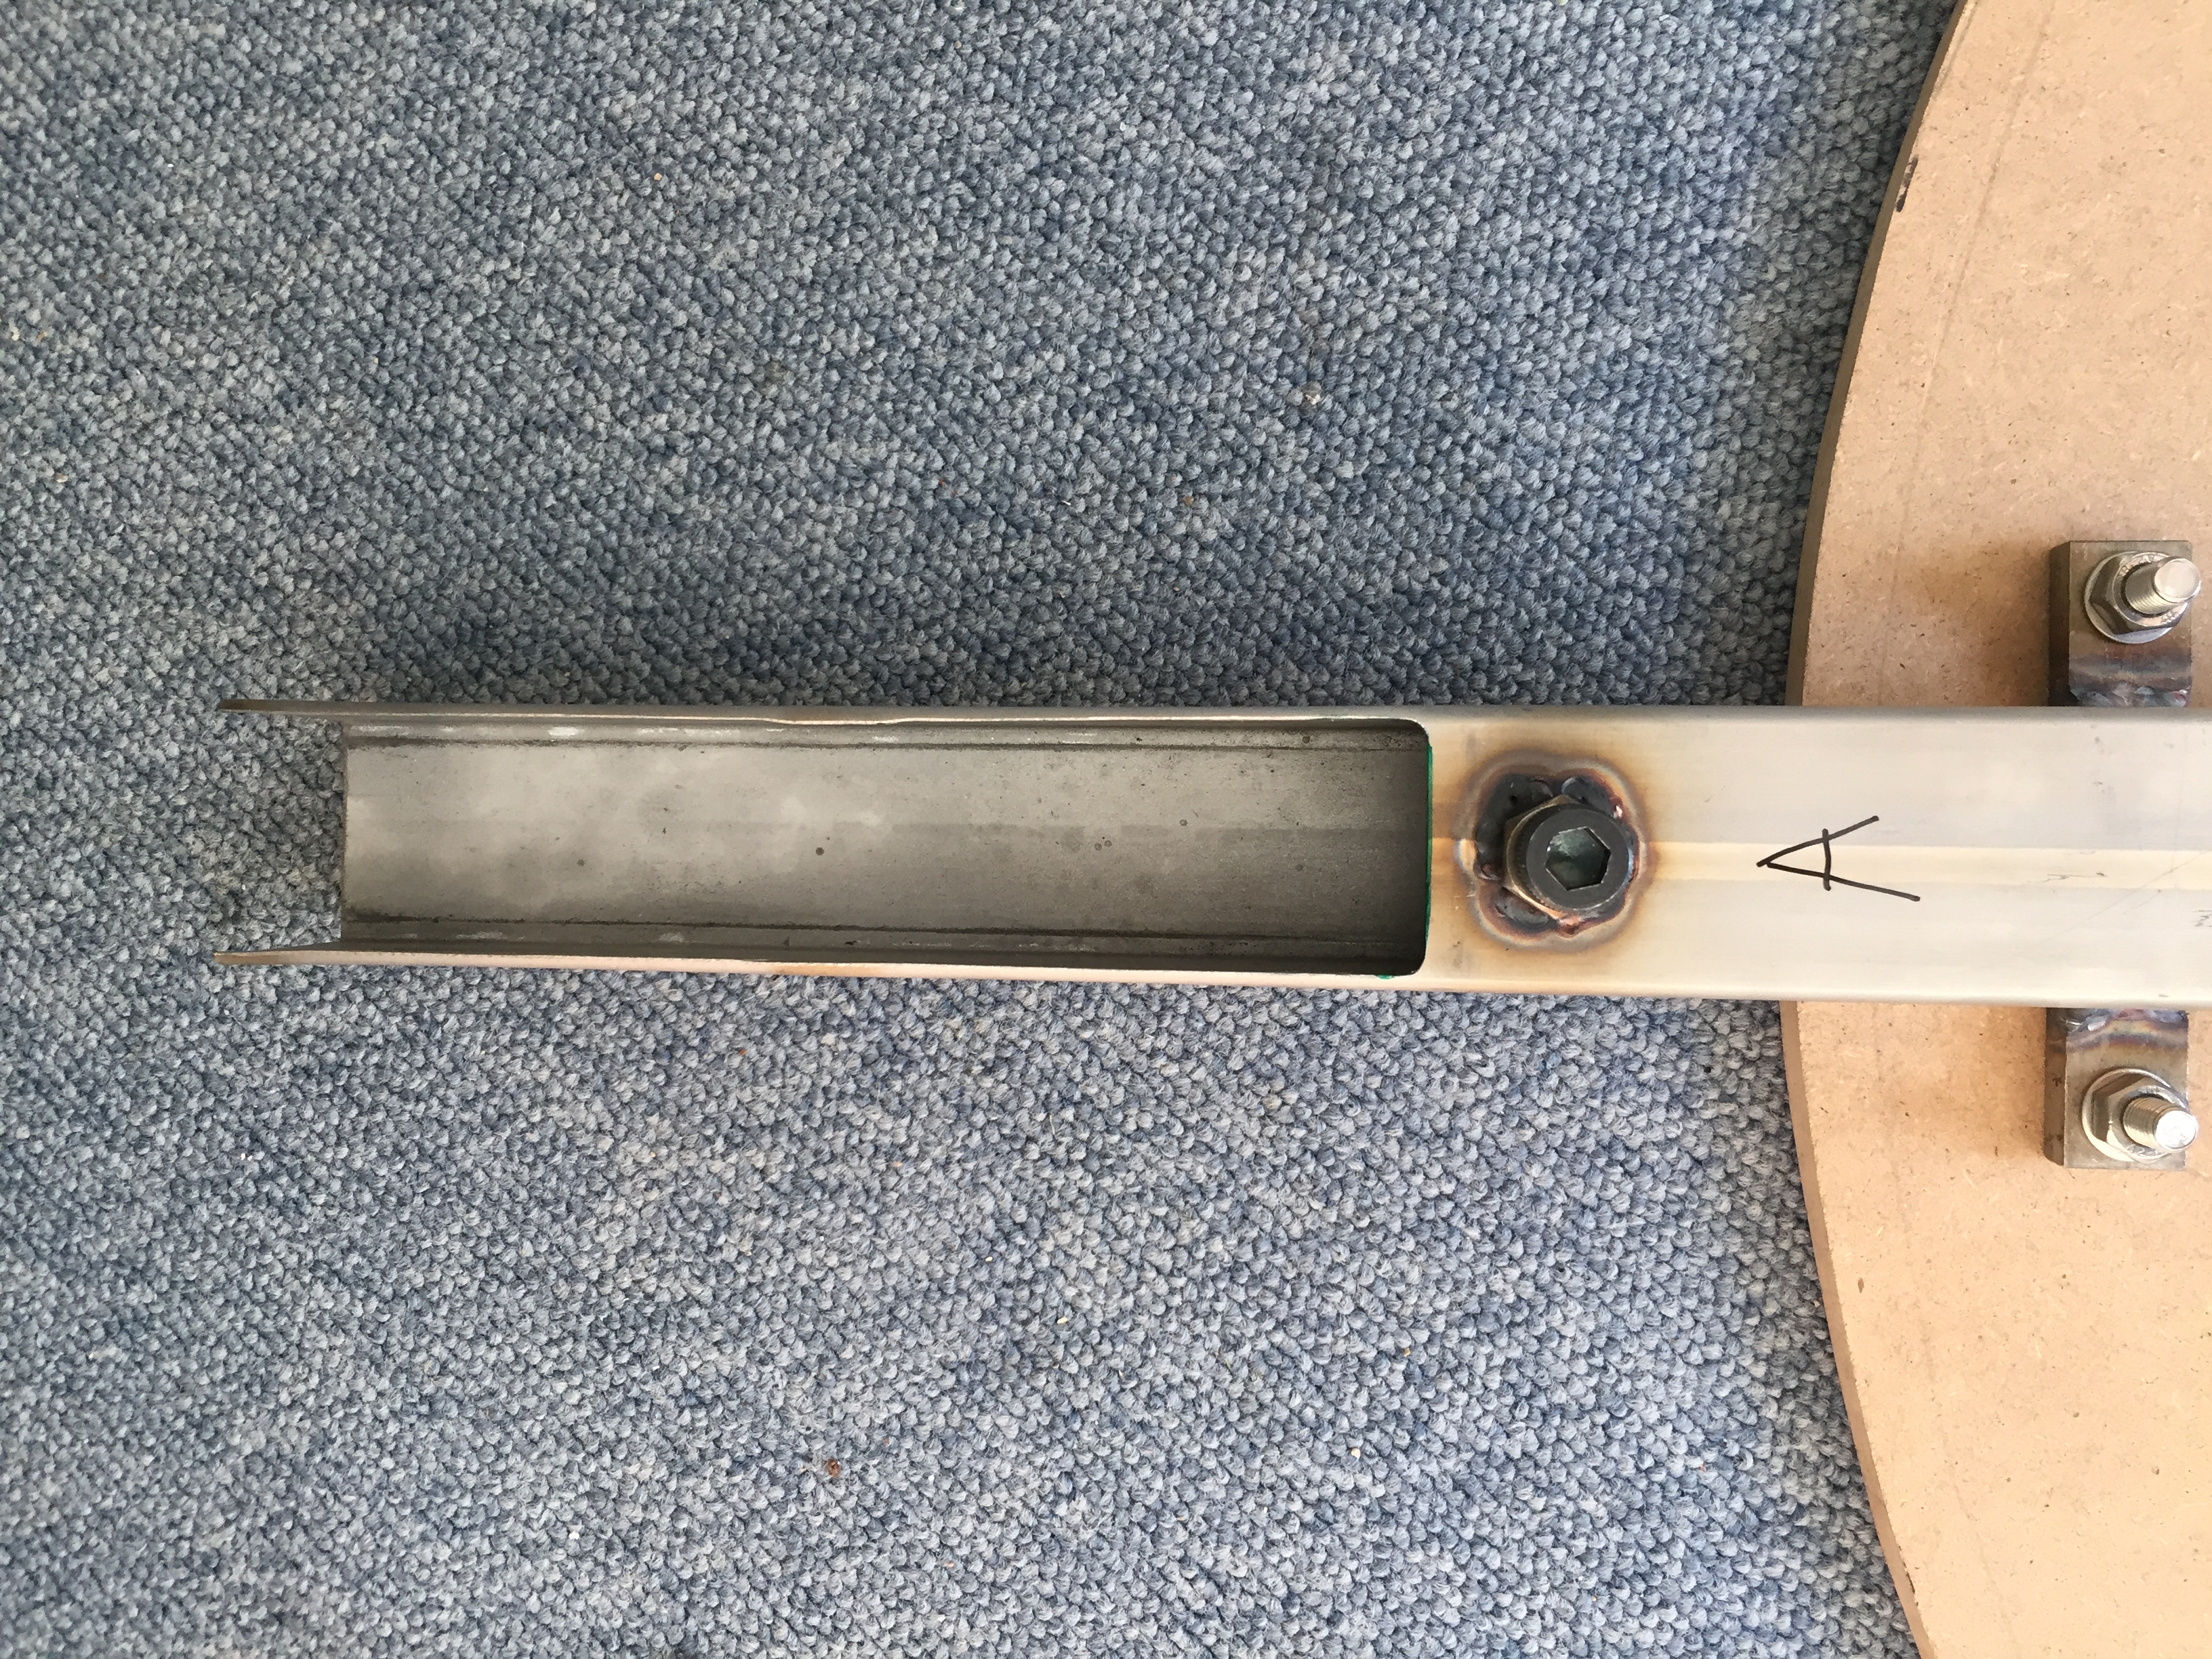
\includegraphics[width=0.5\textwidth]{bottom_u}
	\caption{The bottom part of the speaker stand with the u cut}
		\label{fig:botom_u}
\end{figure}

The speaker have to be placed in a triangle shape, where it is chosen that the centroid is the array center. This placement makes a higher weight at the position where the back speaker is placed compare to the front of the speaker array. Therefore a small plate have to be mounted in the front such that is is possible to mount counter weight to the speaker stand. The final drawing of the bottom part is as \autoref{fig:botom_final}

  \begin{figure}[H]
	\centering
	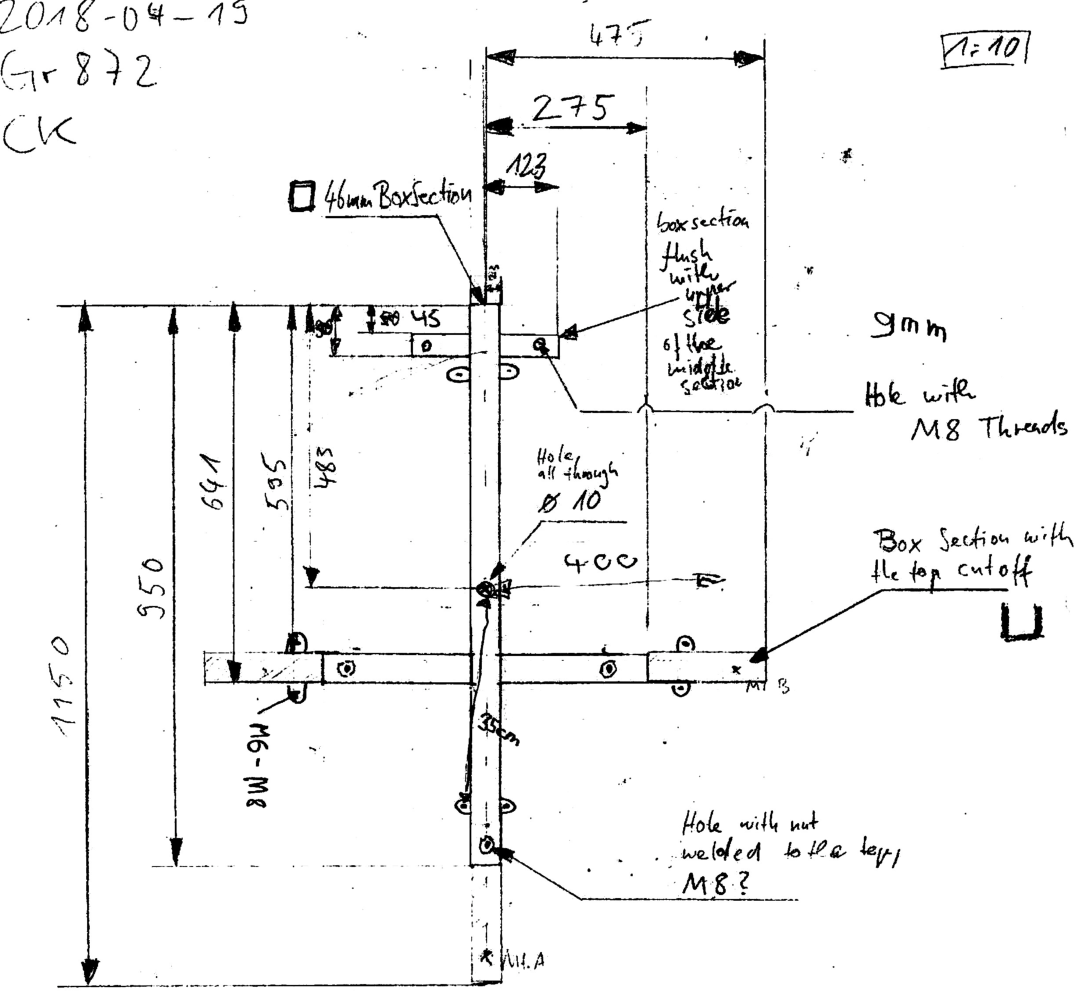
\includegraphics[width=1\textwidth]{bottom_final}
	\caption{A drawing of the bottom part}
		\label{fig:botom_final}
\end{figure}

The corresponding stands is made like a 'L' where the horizontal part of the L can be slided intro the bottom part and the vertical part is used as the hight extender, where the the speaker is mounted on top. The following picture shows the full speaker setup in the anacoid chamber at \gls{aau} \autoref{fig:the_setup}

  \begin{figure}[H]
	\centering
	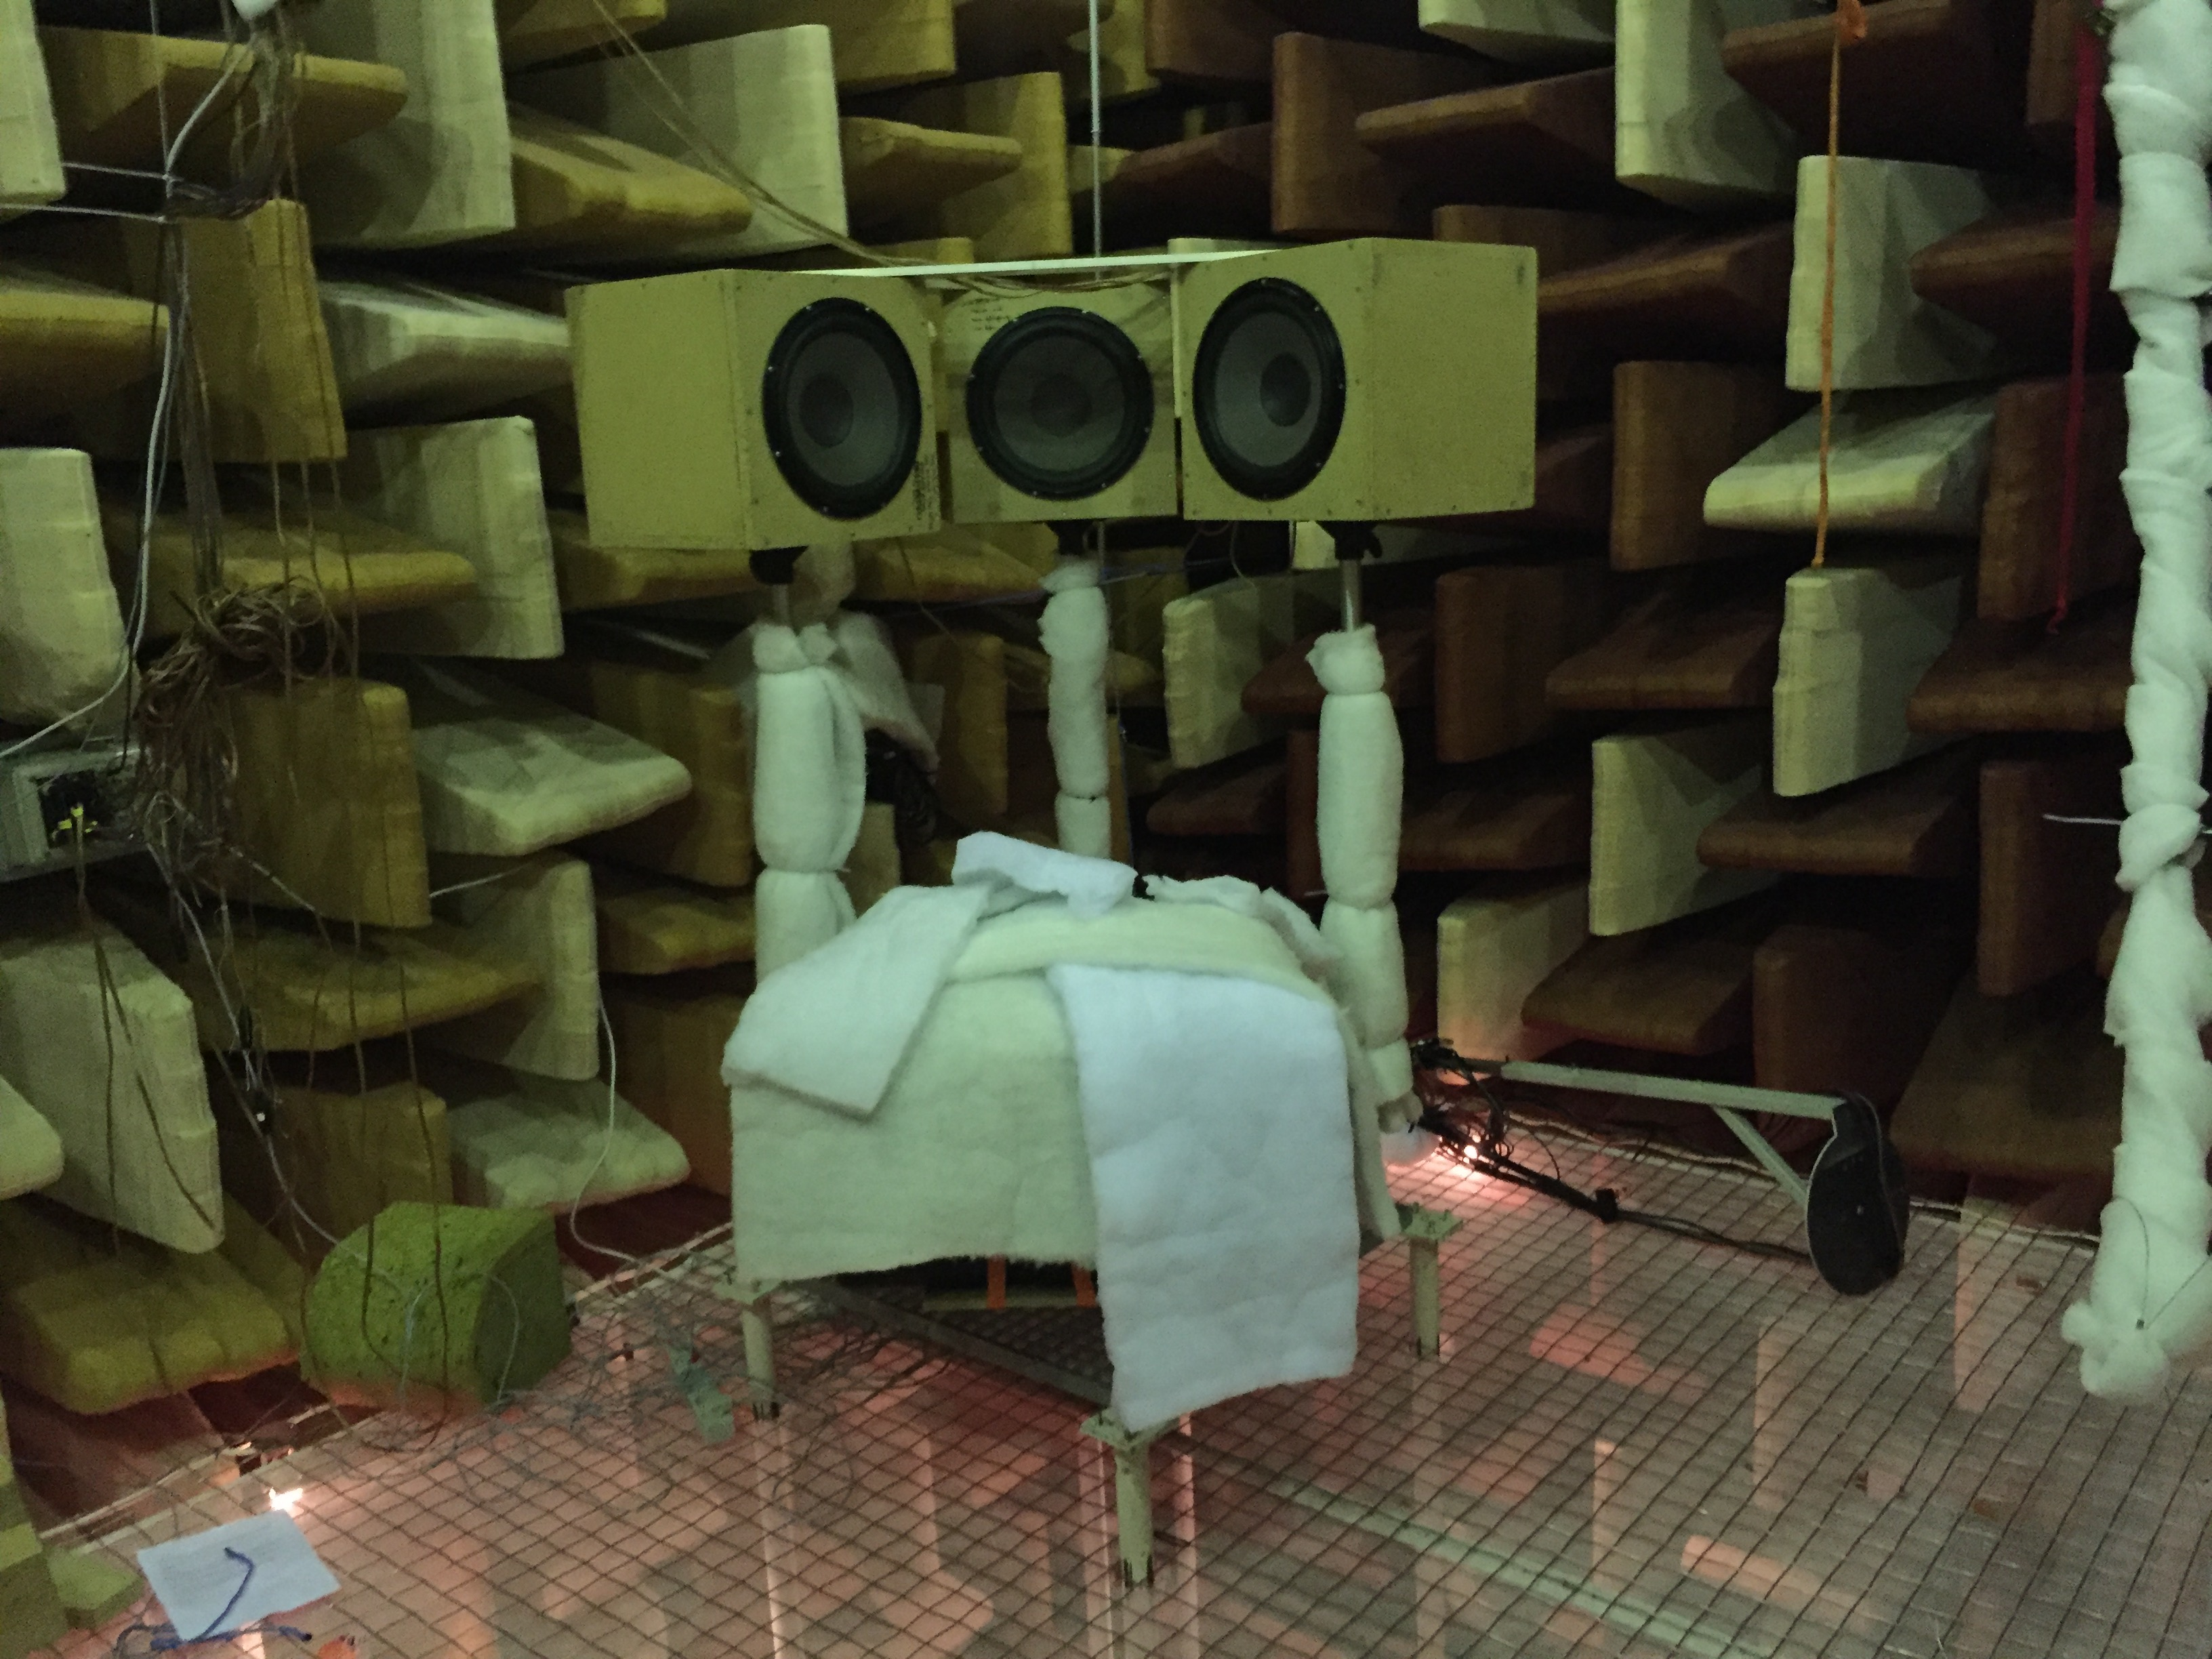
\includegraphics[width=1\textwidth]{the_setup}
	\caption{A picture of the final setup in the anacoid chamber at \gls{aau}}
		\label{fig:the_setup}
\end{figure}

The stiffness of the speaker stand is not rigid enough to hold the speaker at a precise position, and therefore the is build a small triangle wood piece which is mounted on the top on the all speaker. The construction had some oscillate time of \SI{2}{\second} before all speaker is saddled when the turntable stop running, But with the top wood plate, the position of the speaker is exact. 

\section{Conclusion}

It can be concluded that it was possible to make a stable speaker measuring stand where all three speaker can be allined and adjusted and still be a stable construction.




